\documentclass[../ai_in_finance]{subfiles}
\usepackage[margin=1in]{geometry}
\usepackage{tikz}
\usetikzlibrary{positioning,arrows.meta}
\usepackage{amsmath}
\usepackage{amssymb}
\usepackage{booktabs}
\usepackage{floatrow}
\usepackage{draftwatermark}

\SetWatermarkText{Wulin.Suo@Queensu.ca}
\SetWatermarkScale{0.8}
\SetWatermarkColor{gray!35}
\SetWatermarkAngle{0}
\SetWatermarkVerCenter{0.955\paperheight}

\usepackage{makeidx}
\makeindex

\begin{document}

\chapterkey{abm}
\chapter{Agent-Based Models in Finance}

Every model in this book so far has taken one of two forms. Chapter~\chnum{ml}'s machine learning models estimate a function from a fixed dataset, implicitly assuming that the data-generating process does not change while the model learns. Chapter~\chnum{portfolio}'s portfolio theory and Chapter~\chnum{rl}'s reinforcement-learning agents each reason about a single decision-maker, or a small number of them, optimizing against an environment that is either fixed or, at most, adapts slowly.

Neither approach is built to answer a question that matters a great deal in practice: what happens when many participants, each following a simple, individually reasonable rule, interact repeatedly in the same market? Agent-based models\index{agent-based model (ABM)} (ABMs) answer that question. Rather than solving for an equilibrium in closed form or estimating a statistical relationship from historical data, an ABM specifies a population of heterogeneous agents, each governed by a simple behavioral rule, lets them interact in a simulated market, and studies whatever aggregate pattern emerges: a stable price, a bubble, a crash, a cascade of defaults.

This chapter's central claim is that emergence is the point\index{emergence}, not a side effect. Chapter~\chnum{hft}'s account of the 2010 Flash Crash described\index{Flash Crash of 2010!agent-based reconstruction} a version of this: no single participant's inventory-management rule was unreasonable in isolation, yet many such rules operating simultaneously produced a collectively destabilizing 
hot-potato effect that no single participant intended\index{hot-potato effect} or could have predicted from their own rule alone. An ABM can reproduce that kind of 
story directly, agent by agent, rather than only describing it after the fact.

Several worked examples run through this chapter, each reproduced in the companion notebook under the same compute-first
discipline as the rest of the book. A zero-intelligence double-auction example shows that a market mechanism can produce an efficient outcome even when every participant in it behaves close to 
randomly.

A fundamentalist-chartist example shows how the same market can either converge smoothly toward fair value or spiral into a self-reinforcing bubble, depending only on the mix of trading strategies, with no change to the market mechanism, and a 500-period extension shows fat tails and volatility clustering emerging from two simple, fixed behavioral rules switching in and out of dominance. A financial-contagion example, built on the clearing-vector logic behind real central-bank stress-testing models, shows a shock to one institution cascading into the default of a second that was never exposed to the original shock, and a second network topology, compared against the first under the same shock, shows that the same total loss can be concentrated into a few outright defaults or spread thinly across many weakened survivors, depending only on the network's shape.

A final pair of examples previews the AI-driven alternative to fixed-rule agents, developed in Section~\ref{sec:abm-vs-marl}. The first is a seller who learns which of two ask prices is more profitable by trial and error, using Chapter~\chnum{rl}'s Q-learning, and shows the limits of trial-and-error learning when an unlucky early experience locks in the wrong lesson. The second is a fundamentalist-chartist market in which the population mix is switched not by a threshold the modeler imposes but by agents comparing each strategy's recent profit through a discrete-choice rule, so that the bubble-triggering threshold derived earlier is crossed endogenously rather than by assumption.

This places agent-based models among the three modeling paradigms the book has now covered. Chapter~\chnum{ml}'s supervised and unsupervised models answer ``given this data, what function best describes it,'' and are validated by predictions on data the model never saw. Chapter~\chnum{rl}'s reinforcement-learning agents answer ``given this environment, what sequence of actions maximizes reward,'' and are validated by realized performance, in a backtest or in production.

Agent-based models answer a third question: ``given these individual rules, what pattern emerges when many such agents interact,'' and, as Section~\ref{sec:abm-calibration} develops, they are validated far more weakly than the other two, by whether a simulated pattern resembles an observed one rather than by a held-out prediction or a realized return. None of the three is more fundamentally correct; they answer different questions, and recognizing which question a financial problem poses (prediction, sequential decision, or emergence) is one of this book's recurring practical lessons. Table~\ref{tab:abm-paradigms} lays the three side by side.

\begin{booktable}[htbp]{Three modeling paradigms used in this book}{tab:abm-paradigms}
\begin{tabular}{L{2.4cm}L{4.5cm}L{3.4cm}L{4.3cm}}
\toprule
 & Supervised/\allowbreak unsupervised ML (Ch.~\chnum{ml}) & Reinforcement learning (Ch.~\chnum{rl}) & Agent-based models (this chapter) \\
\midrule
Core question & What function best fits this data? & What action sequence maximizes reward? & What pattern emerges from many interacting rules? \\
Input & A fixed, historical dataset & An environment to interact with & A set of behavioral rules and a market mechanism \\
Validation & Held-out prediction accuracy & Realized backtest or live performance & Resemblance to observed stylized facts (weakest of the three) \\
Typical output & A trained predictive model & A trained policy & A simulated history and its emergent statistics \\
\bottomrule
\end{tabular}
\end{booktable}

A reader who has followed this book's emphasis on machines that learn might object that every rule above, zero-intelligence, fundamentalist, chartist, is fixed by the modeler in advance, which sits oddly in a book about AI in finance. The fixed-rule design is a deliberate methodological choice, not a limitation of agent-based modeling, and it keeps Table~\ref{tab:abm-paradigms}'s third column honest: separating the question of what pattern emerges from a given set of rules from the question of how an agent's rule might itself be learned keeps each worked example small enough to hand-check, the discipline Chapters~\chnum{intro} through~\chnum{rl} apply everywhere else.

That second question, learning the rule itself, is Chapter~\chnum{rl}'s question, and Section~\ref{sec:abm-vs-marl} connects the two. It argues that agent-based models and multi-agent reinforcement learning (MARL) are two responses to the limitation Chapter~\chnum{rl} identifies in its own single-agent framing, that training a policy against a fixed historical simulator assumes every other participant's behavior stays fixed, and it makes the connection concrete through the learning-seller example previewed above, in which one agent in an otherwise fixed-rule market learns its own quoting rule with Chapter~\chnum{rl}'s Q-learning. Every fixed-rule agent elsewhere in the chapter is a transparent, tractable special case of that more general world, in which agents learn rather than follow a rule handed to them and which is much harder to train and validate, not a rejection of it.

Each application follows the same escalating structure: state the mechanism and a small, hand-checkable illustration, then show what happens when the mechanism is scaled up or repeated. Sections~\ref{sec:abm-zi} and~\ref{sec:abm-fundamentalist-chartist} build market-level price dynamics from individual trading rules; Section~\ref{sec:abm-stylized-facts} scales the latter to hundreds of periods to show statistical patterns emerging; Sections~\ref{sec:abm-contagion} and~\ref{sec:abm-advanced} apply the same logic to a network of banks. Section~\ref{sec:abm-vs-marl} compares the fixed-rule agents with Chapter~\chnum{rl}'s learned alternative, and Section~\ref{sec:abm-workflow} distills the common workflow into a reusable template. The chapter closes with the practical limitations, summarized in Section~\ref{sec:abm-calibration} and the Challenges section, that keep agent-based models a specialized complement to the book's other methods rather than a replacement for them.

\section{Why Agent-Based Models}

Replacing the representative agent with many heterogeneous ones changes what a model can produce.

\subsection{From Representative Agents to Heterogeneous, Interacting Ones}
\label{sec:abm-why}\index{heterogeneous agents}

Much of classical finance, and much of this book, reasons in terms of a representative agent\index{representative agent}: Chapter~\chnum{portfolio}'s CAPM derives an equilibrium as though a single, rational, mean-variance investor stood in for the whole market; Chapter~\chnum{timeseries}'s GARCH models fit a single statistical process to an entire return series without asking which market participants' behavior produced that process. These simplifications are enormously useful, and this book relies on them throughout, but by construction they cannot answer certain questions.

A representative-agent model cannot easily explain why a market that is efficient on an average day can suffer a Flash Crash on a particular afternoon, because the average behavior built into the model has already smoothed away the heterogeneity that made the crash possible. Agent-based modeling starts at the other end: instead of solving for what a single rational agent would do, it specifies what a population of different, typically boundedly rational, agents do, and asks what pattern emerges from their interaction.

This bottom-up approach is well suited to the phenomena that are hardest to explain with a representative agent: the fat tails and volatility clustering Chapter~\chnum{timeseries}'s GARCH models describe statistically\index{stylized facts} but do not explain mechanistically; asset-price bubbles and crashes that unfold over time\index{bubble} rather than instantaneously; and the kind of systemic, contagious risk\index{systemic risk} Chapter~\chnum{marketrisk}'s stress-testing framework treats largely at the level of a single institution's portfolio rather than as a property of an interconnected system.

Agent-based modeling did not originate in finance. Its most famous early instance is the segregation model of \textcite{schelling1971dynamic}\index{Schelling segregation model}, built with a checkerboard and coins of two colors: each agent mildly prefers to have at least some same-type neighbors, far short of wanting a segregated neighborhood, and moves to a nearby empty square only if that preference is unmet. Simulating this individually reasonable rule across many agents produces, almost without exception, a starkly segregated checkerboard, an outcome none of the agents asked for. The financial applications in this chapter apply the same logic to markets: individually reasonable rules, simulated across many interacting agents, produce an aggregate outcome (efficiency, a bubble, a cascade of defaults) that is a property of the interaction rather than of any agent's intentions.

The idea reached finance through the Santa Fe Institute's Artificial Stock Market\index{Santa Fe Artificial Stock Market}, built in the early 1990s by Arthur, Holland, LeBaron, Palmer, and Tayler and described in \textcite{arthur1997asset}, widely regarded as the first serious agent-based model of a financial market. Instead of the two fixed strategy types of Section~\ref{sec:abm-fundamentalist-chartist}'s model, its agents carried evolving collections of predictive rules, more like a population of competing forecasting models, and poorly performing rules died out while successful ones proliferated, an early instance of the performance-based selection Brock and Hommes later formalized more tractably. Its central finding, that the market could switch between a calm, efficient regime and a volatile, trend-chasing regime\index{regime switching} depending on how quickly agents adapted their rules, foreshadows the mechanism behind Section~\ref{sec:abm-stylized-facts}'s worked example, and the project is credited with establishing agent-based computational finance as a research area separate from the social-science tradition of Schelling's model.

Agent-based models now play a recurring role in the finance industry, which this chapter's later sections examine. Central banks and other macroprudential regulators run network-based models\index{systemic risk!stress testing} with behavioral feedbacks, such as the Bank of England's RAMSI in the case vignette below, to stress-test a banking system's interconnected exposures rather than one institution at a time, now a standard part of the macroprudential toolkit. Exchanges and microstructure researchers use zero-intelligence and heterogeneous-agent markets, the subject of Sections~\ref{sec:abm-zi} and~\ref{sec:abm-fundamentalist-chartist}, to learn how much of observed market efficiency, or its breakdown in an event like the Flash Crash, comes from the trading mechanism rather than from participants' sophistication. Quantitative trading desks build synthetic, agent-populated limit-order-book markets\index{market simulator} to test how a new execution algorithm of the kind Chapter~\chnum{algotrading} develops is likely to move prices and interact with others before risking capital on it, a cheaper and safer proving ground than live trading. And a growing body of research combines agent-based markets with the multi-agent reinforcement learning of Section~\ref{sec:abm-vs-marl}, training an execution or market-making policy inside a simulated population of agents rather than against static historical data alone.

Figure~\ref{fig:abm-loop} sketches the simulation loop every example in this chapter follows: a population of agents, each with its own rule, observes the market state; each agent acts (submits an order, updates a belief, decides whether to pay a debt); a market mechanism aggregates the actions into a new state; and the loop repeats. Nothing is estimated from historical data the way Chapter~\chnum{ml}'s models are; everything is specified as a rule and simulated forward.

\begin{bookfigure}[htbp]{The basic agent-based simulation loop}{fig:abm-loop}
    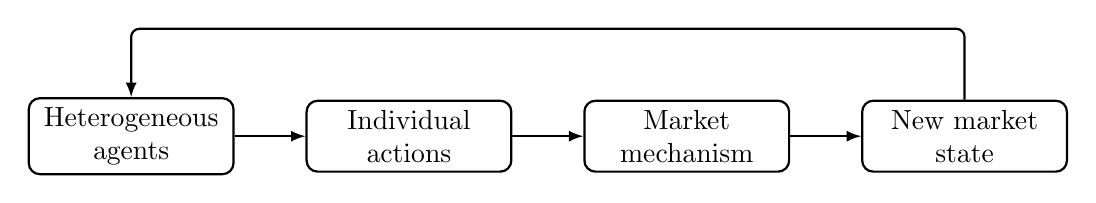
\begin{tikzpicture}[>=latex,thick,node distance=0.9cm]
        \node[draw,rounded corners,minimum width=2.6cm,minimum height=0.9cm,align=center] (agents) {Heterogeneous\\agents};
        \node[draw,rounded corners,minimum width=2.6cm,minimum height=0.9cm,right=of agents,align=center] (actions) {Individual\\actions};
        \node[draw,rounded corners,minimum width=2.6cm,minimum height=0.9cm,right=of actions,align=center] (market) {Market\\mechanism};
        \node[draw,rounded corners,minimum width=2.6cm,minimum height=0.9cm,right=of market,align=center] (state) {New market\\state};
        \draw[->] (agents) -- (actions);
        \draw[->] (actions) -- (market);
        \draw[->] (market) -- (state);
        % Orthogonal feedback route rather than a bezier arc: a to[out=135,in=45]
        % curve bulges in proportion to the chain's width, and across four boxes it
        % claimed more vertical space than the boxes themselves. This rises a fixed
        % 0.9cm whatever the chain's width (0.5cm read as running along the box tops). Same fix as Chapter 6's lifecycle figure.
        \draw[->,rounded corners=3pt] (state.north) -- ++(0,0.9) -| (agents.north);
    \end{tikzpicture}
\end{bookfigure}

\subsection{Zero-Intelligence Traders and the Double Auction}
\label{sec:abm-zi}\index{double auction}

The most striking early result in agent-based market modeling, due to \textcite{gode1993allocative}\index{Gode-Sunder zero-intelligence model}, is that a double auction, the continuous matching of bids against asks behind the limit order book of Chapter~\chnum{markets}\index{limit order book}, can produce a highly efficient outcome even when no trader in it is intelligent at all: a ``zero-intelligence'' trader submits a bid or ask drawn at random\index{zero-intelligence traders} from a budget-feasible range, with no strategic reasoning about price or other traders. Consider two buyers with private valuations $V_{B1}=\$52$ and $V_{B2}=\$48$, and two sellers with private costs $C_{S1}=\$45$ and $C_{S2}=\$50$, for one unit of the same asset each. The efficient allocation, the one a fully rational market would produce, is easy to find: buyer 1 and seller 1 should trade, since $V_{B1} > C_{S1}$ generates a surplus of $52-45=\$7$, while buyer 2 and seller 2 should not, since $V_{B2} < C_{S2}$ would destroy value. Total efficient surplus is therefore $\$7$.

Now suppose each buyer $i$ submits a random bid drawn from $[0, V_{Bi}]$ and each seller $j$ a random ask drawn from $[C_{Sj}, 100]$, ranges that keep each trader budget-feasible (a buyer never bids above its valuation, a seller never asks below its cost), with $\$100$ an arbitrary price ceiling. Nobody knows anyone else's valuation. Suppose that in one simulated round the draws are $b_1=\$50$ (buyer 1), $b_2=\$30$ (buyer 2), $a_1=\$47$ (seller 1), and $a_2=\$65$ (seller 2). The standard double-auction clearing rule sorts bids from highest to lowest and asks from lowest to highest, then matches and trades every pair whose bid meets or exceeds the ask:
\begin{align*}
\text{Bids (descending):} &\quad 50, \ 30, \\
\text{Asks (ascending):} &\quad 47, \ 65.
\end{align*}
The top bid, $\$50$, meets the top ask, $\$47$ ($50 \ge 47$), so buyer 1 and seller 1 trade; the second bid, $\$30$, does not meet the second ask, $\$65$ ($30 < 65$), so buyer 2 and seller 2 do not. By matching random bids against random asks, the clearing mechanism has selected the efficient pair, buyer 1 with seller 1, and rejected the inefficient one. Whatever transaction price rule is used, for instance the midpoint of the matched bid and ask, $(50+47)/2 = \$48.5$, the realized surplus, computed from true valuations rather than random bids, is $V_{B1} - C_{S1} = 52 - 45 = \$7$, the full efficient surplus, captured although neither trader bid or asked anything close to its true valuation. The lesson, confirmed systematically in Gode and Sunder's experiments across many traders and rounds, is that a market's efficiency can come largely from the structure of the trading mechanism\index{market efficiency}\index{market design} rather than from the sophistication of its traders, a counterintuitive result relative to the fully rational representative agent of Chapter~\chnum{portfolio}'s equilibrium models. This single round shows that the mechanism \emph{can} select the efficient pair from random bids, not that it \emph{always} will. As the companion notebook's supplementary experiments with this two-buyer, two-seller market confirm, a single random draw from a wide range is a noisy way to reach that outcome; Gode and Sunder's robust result relies on many traders and many trading opportunities per period, not on one exchange like the one worked above.

\subsection{Building a Simple ABM in Python}
\label{sec:abm-python}\index{agent-based model (ABM)!building in Python}

Every agent-based model in this chapter reduces to two ingredients Chapter~\chnum{python} already teaches how to code: a data structure for each agent's state, and a function that updates the market given every agent's action. The zero-intelligence double auction above takes only a few lines:
\begin{verbatim}
import random

def zero_intelligence_round(buyers, sellers, seed=None):
    rng = random.Random(seed)
    bids = [(rng.uniform(0, v), v) for v in buyers]      # random bid, true value
    asks = [(rng.uniform(c, 100), c) for c in sellers]    # random ask, true cost
    bids.sort(key=lambda x: -x[0])
    asks.sort(key=lambda x: x[0])
    trades = []
    for (bid, val), (ask, cost) in zip(bids, asks):
        if bid >= ask:
            trades.append({'price': (bid + ask) / 2, 'surplus': val - cost})
    return trades

trades = zero_intelligence_round(buyers=[52.0, 48.0], sellers=[45.0, 50.0], seed=2)
print(trades)   # [{'price': 48.91, 'surplus': 7.0}]
\end{verbatim}
Every other example in the chapter follows the same pattern: Section~\ref{sec:abm-fundamentalist-chartist}'s price dynamics are a one-line update rule called in a loop; Section~\ref{sec:abm-contagion}'s clearing vector is a short function computing each bank's payment given what it receives; and Section~\ref{sec:abm-stylized-facts}'s 500-period simulation is the same fundamentalist-chartist loop with an \texttt{if} statement selecting each period's regime. None of this needs tools beyond Chapter~\chnum{python}; what distinguishes agent-based modeling is not the code but the habit of specifying individual rules and letting the population-level pattern emerge from running them, rather than solving for it in closed form. The brevity matters: it is what makes a fixed-rule agent fully interpretable, since each of these short functions is a rule a reader can audit line by line, as a Chapter~\chnum{rl} policy's learned weights are not, a contrast Section~\ref{sec:abm-vs-marl} develops once both approaches are on the table.

This is also why the companion notebook, not the chapter text, is the place to explore an ABM's behavior. Each worked example reports one set of parameter values and, where relevant, one random seed. Changing any of them (the switching threshold, the population shares, the interbank network's shape, the buyer valuations the learning seller faces) produces a different simulated history, and the only way to build intuition for how sensitive a result is to an assumption is to make the change and rerun, the hands-on exploration this book's preface encourages for every companion notebook.

\subsection{Heterogeneous Agents, Bubbles, and Crashes: Fundamentalists versus Chartists}
\label{sec:abm-fundamentalist-chartist}\index{fundamentalists and chartists}\index{heterogeneous agents}

Zero-intelligence traders show that a market mechanism can be efficient despite unsophisticated participants; they do not explain bubbles and crashes, since random bidding has no memory and no tendency to extrapolate a trend. The next step in the agent-based tradition, associated with Brock and Hommes\index{Brock-Hommes model} and with Lux and Marchesi\index{Lux-Marchesi model}, introduces two purposeful agent types whose population shares can shift over time. In plain terms, a fundamentalist behaves like a value investor: the further the price sits below what the asset is worth, the more eagerly the fundamentalist buys, and the further above, the more eagerly it sells, a demand rule that always leans toward pulling the price back to fundamental value. A chartist behaves like a momentum trader\index{trend following}: the faster the price has just risen, the more eagerly the chartist buys, betting that the trend continues, with no opinion about what the asset is worth. Formally, fundamentalists believe the price will revert toward a known fundamental value $p_f$ and submit demand proportional to the mispricing,
\begin{equation}
d^f_t = \alpha (p_f - p_t),
\label{eq:abm-fundamentalist}
\end{equation}
while chartists (trend followers) extrapolate the most recent price change forward, submitting demand proportional to recent momentum,
\begin{equation}
d^c_t = \beta (p_t - p_{t-1}).
\label{eq:abm-chartist}
\end{equation}
A simple market-impact rule aggregates the two populations' demand, weighted by their respective population shares $n_f$ and $n_c = 1-n_f$, into a single aggregate demand,
\begin{equation*}
D_t = n_f\, d^f_t + n_c\, d^c_t,
\end{equation*}
which a linear price-impact equation converts into a price update\index{market impact},
\begin{equation}
p_{t+1} = p_t + \lambda D_t,
\label{eq:abm-price-update}
\end{equation}
where $\lambda$ controls how strongly aggregate demand moves the price. The ``Aggregate demand'' column of Table~\ref{tab:abm-scenario-a} below reports $D_t$ at each step. The fundamental value, the two behavioral rules, and the price-impact equation are held fixed across the two scenarios below; only the population mix $(n_f, n_c)$ differs.

\weheading{\subsubsection*}{abm-bubble}{Convergence versus a Self-Reinforcing Bubble}\index{fundamentalists and chartists!bubble and crash}\index{bubble}

Let $p_f = 100$, $\alpha = 0.3$, $\beta = 1.0$, $\lambda = 1.5$, and start both scenarios from the same two initial prices, $p_{-1} = \$93$ and $p_0 = \$95$ (a modest existing uptrend). In Scenario A, fundamentalists are the large majority, $n_f = 0.8$, $n_c = 0.2$. Table~\ref{tab:abm-scenario-a} works the first three steps by hand.

\begin{booktable}[htbp]{Scenario A: fundamentalist-dominated market ($n_f=0.8$, $n_c=0.2$), converging toward $p_f=100$}{tab:abm-scenario-a}
\begin{tabular}{lrrrrr}
\toprule
$t$ & $p_t$ & $d^f_t$ & $d^c_t$ & Aggregate demand $D_t$ & $p_{t+1}$ \\
\midrule
0 & 95.000 & 1.500 & 2.000 & 1.600 & 97.400 \\
1 & 97.400 & 0.780 & 2.400 & 1.104 & 99.056 \\
2 & 99.056 & 0.283 & 1.656 & 0.558 & 99.893 \\
\bottomrule
\end{tabular}
\end{booktable}

The price rises from $\$95.00$ toward the fundamental value of $\$100$ in shrinking steps, $\$2.40$, then $\$1.66$, then $\$0.84$: the damped convergence a stabilizing fundamentalist majority should produce, since the fundamentalist demand pulling the price toward $p_f$ weakens as the price approaches it.

Scenario B changes only the population mix, to a market with no fundamentalists at all, $n_f = 0$, $n_c = 1$. With $n_f=0$ the price update collapses to $p_{t+1} = p_t + \lambda\beta(p_t - p_{t-1})$, and since $\lambda\beta = 1.5 \times 1.0 = 1.5 > 1$, each period's price change is $1.5$ times the previous one, an explosive recursion with no anchor to $p_f$:
\begin{align*}
p_1 &= 95 + 1.5(95-93) = 95 + 3.00 = 98.00, \\
p_2 &= 98 + 1.5(98-95) = 98 + 4.50 = 102.50, \\
p_3 &= 102.5 + 1.5(102.5-98) = 102.5 + 6.75 = 109.25.
\end{align*}
The price moves further from the fundamental value of $\$100$ every period, by $\$3.00$, then $\$4.50$, then $\$6.75$, a self-reinforcing bubble driven by momentum-chasing, with each move larger than the last. The market mechanism did not change between Scenario A and Scenario B; only the composition of the trading population did. This kind of regime-dependent behavior, stable in one population mix and explosive in another, is what a single representative agent cannot produce\index{representative agent}, since a representative agent is always the same agent.

\subsection{Why the Market Tips: A General Stability Condition}
\label{sec:abm-stability}\index{fundamentalists and chartists!stability condition}

Scenario A converged and Scenario B exploded, but they also differed in $n_c$, which raises the question of how much chartist weight tips the market from one regime to the other. The answer is the kind of population-level fact this chapter keeps returning to. It is written into neither behavioral rule, since neither demand equation mentions a critical population share, yet their combination produces a sharp, calculable threshold that a representative-agent model could not even pose, having no population mix to vary (Section~\ref{sec:abm-why}). Intuitively, a chartist's demand today depends on how much the price just rose, but that demand also pushes the price up tomorrow, feeding a fresh, possibly larger, round of chartist demand the day after; whether the loop fizzles out or feeds on itself depends on its strength relative to the fundamentalist demand pulling the other way, a balance the threshold below makes precise. Substituting the two demand equations into the price-update rule turns the model into a linear recursion in the
two most recent prices alone,
\begin{equation}
p_{t+1} = \lambda n_f\alpha p_f + (1-\lambda n_f\alpha+\lambda n_c\beta)\,p_t - \lambda n_c\beta\,p_{t-1},
\label{eq:abm-recursion}
\end{equation} 
and the standard stability analysis for a recursion of this form (worked out in full, and confirmed against a parameter sweep, 
in the companion notebook) shows that, for every parameter combination used in this section, the market is stable if and only if
\begin{equation}
\lambda n_c \beta < 1.
\label{eq:abm-stability}
\end{equation}
Scenario A's coefficient was $\lambda n_c \beta = 1.5 \times 0.2 \times 1.0 = 0.30 < 1$, comfortably stable; Scenario B's, with no fundamentalists diluting the chartist share at all, was $\lambda n_c \beta = 1.5 \times 1.0 \times 1.0 = 1.50 > 1$, explosive. Solving $\lambda n_c \beta = 1$ for the population share gives the exact critical threshold,
\begin{equation*}
n_c^{*} = \frac{1}{\lambda \beta} = \frac{1}{1.5 \times 1.0} \approx 0.667,
\end{equation*}
so this market tips from convergent to explosive once chartists exceed roughly two-thirds of the trading population, holding $\lambda$ and $\beta$ at the values used throughout this section. The companion notebook confirms the threshold: at $n_c=0.60$, just below $n_c^{*}$, the price oscillates around $p_f$ with shrinking amplitude, settling close to $\$100$ within about $60$ periods, while at $n_c=0.70$, just above $n_c^{*}$, it oscillates with growing amplitude, reaching $87.7$ after only $15$ periods and still widening. Near the threshold, convergence is oscillatory rather than the smooth, monotonic approach of Scenario A's $n_c=0.2$, because the recursion's roots are a complex-conjugate pair whenever $n_c$ is this large: the market converges not just more slowly but differently, overshooting $p_f$ and swinging back before settling. This kind of sharp regime change, a market that behaves completely differently once one parameter crosses a critical value, motivates the endogenous switching mechanism behind\index{regime switching} Section~\ref{sec:abm-stylized-facts}'s simulation: real markets do not sit at a fixed $n_c$, and a population that drifts back and forth across a threshold like $n_c^{*}$ alternates between the qualitatively different regimes worked out above.

\section{Emergence and Systemic Risk}

The point of these models is what they produce without being told to, including contagion nobody designed.

\subsection{Emergent Stylized Facts: Fat Tails and Volatility Clustering from Simple Rules}
\label{sec:abm-stylized-facts}\index{stylized facts!fat tails}\index{stylized facts!volatility clustering}

Chapter~\chnum{timeseries}'s GARCH(1,1) model captures\index{GARCH model} volatility clustering\index{volatility clustering} by imposing an autoregressive structure on the variance of returns: large moves tend to follow large moves because the model's parameters say so. Heterogeneous agent models like Section~\ref{sec:abm-fundamentalist-chartist}'s reproduce the same stylized fact, along with the excess kurtosis (fat tails)\index{fat tails} Chapter~\chnum{timeseries} discusses when introducing GARCH, without specifying any variance process. Suppose the population mix $(n_f, n_c)$ evolves over time, shifting toward chartists whenever chartist strategies have recently been more profitable, the performance-based strategy switching Brock and Hommes formalize\index{Brock-Hommes model}. The market then alternates endogenously between calm, fundamentalist-dominated periods like Scenario A and volatile, chartist-dominated episodes like Scenario B, and clustered volatility and heavy-tailed returns emerge from the switching itself rather than from an assumption built into the model. The distinction matters in practice: a GARCH model is a superb tool for forecasting volatility once fitted, Chapter~\chnum{timeseries}'s use case, but it does not explain why volatility clusters, while an agent-based model offers one candidate mechanism, at the cost of being much harder to fit confidently to a historical dataset, a tension Section~\ref{sec:abm-calibration} returns to.

\weheading{\subsubsection*}{abm-vol-clustering}{Volatility Clustering from Endogenous Regime Switching}\index{volatility clustering!emergent, in agent-based models}\index{regime switching}

The companion notebook makes this concrete by extending the fundamentalist-chartist model to $500$ simulated periods, with two bounded (non-explosive) regimes rather than Scenario B's deliberately unbounded pure-chartist case: a calm regime ($n_f=0.85$, $n_c=0.15$, normally distributed price shocks with standard deviation $0.15$) and a volatile regime ($n_f=0.25$, $n_c=0.75$, shock standard deviation $0.50$), each added to the price update of equation~\eqref{eq:abm-price-update}. The simulation keeps $\alpha=0.3$ and $p_f=100$ but uses $\beta=1.1$ and $\lambda=1.0$, not the $\beta=1.0$ and $\lambda=1.5$ of Section~\ref{sec:abm-fundamentalist-chartist}, and the difference matters: by condition~\eqref{eq:abm-stability}, Section~\ref{sec:abm-fundamentalist-chartist}'s values would give the volatile regime $\lambda n_c\beta = 1.5\times0.75\times1.0 = 1.125 > 1$, an explosive market, whereas the simulation's values give $1.0\times0.75\times1.1 = 0.825$ in the volatile regime and $0.165$ in the calm one, both safely below $1$. The simulation switches into the volatile regime whenever the most recent price move exceeds a fixed threshold, a simple proxy for a situation in which a chartist strategy would just have outperformed a fundamentalist one, and reverts to the calm regime otherwise. Both regimes are individually stable: the price never diverges the way Scenario B's pure-chartist market did, ranging from $\$93.93$ to $\$107.77$ over the full $500$ periods. But the two regimes' realized volatility differs sharply. The simulation spends $213$ periods in the calm regime, with a return variance of $0.147$, and $287$ periods in the volatile regime, with a return variance of $0.903$, a variance ratio of $6.14\times$ between two regimes driven by the same shock process and differing only in which population of traders is active. The full 500-period return series has a Pearson kurtosis of $4.67$, well above the Gaussian benchmark of $3.0$ (an excess kurtosis of $1.67$), confirming fat tails\index{fat tails}, and the autocorrelation of squared returns\index{autocorrelation}, the standard volatility-clustering diagnostic Chapter~\chnum{timeseries} applies to real return series, is $0.658$ at a lag of one period and still $0.216$ at a lag of five, both far from the zero that i.i.d.\ returns would produce. None of these statistics (the variance ratio, the excess kurtosis, the squared-return autocorrelation) was a modeling target; all three emerged from a simulation whose only design choice was which population of fixed behavioral rules was active each period.

\subsection{Agent-Based Models of Systemic Risk and Financial Contagion}
\label{sec:abm-contagion}\index{contagion}\index{systemic risk!contagion}

The examples so far model a single market's price. A separate application, and for regulators arguably a more important one, models a financial system of interconnected institutions, extending Chapter~\chnum{marketrisk}'s stress-testing framework from a single portfolio to a network\index{stress testing!network}. The idea is intuitive: if a bank cannot pay all it owes, every bank counting on that payment is now short of cash, and may in turn be unable to pay everyone counting on \emph{it}, so one institution's shortfall can pass through a network of obligations to institutions that never dealt with the original problem. \textcite{eisenberg2001systemic}\index{Eisenberg-Noe clearing model} formalize this chain reaction as a clearing vector: given a network of interbank obligations and each bank's external (non-interbank) assets, compute how much each bank actually pays, recognizing that a bank not paid in full by others may be unable to pay its own obligations in full. Writing $\bar p_i$ for bank $i$'s total interbank obligation, $e_i$ for its external assets, and $\pi_{ji}$ for the fraction of bank $j$'s obligations owed to bank $i$, the clearing vector $p$ solves
\begin{equation}
p_i = \min\Big(\bar p_i,\; e_i + \sum_j \pi_{ji}\, p_j\Big) \quad \text{for every bank } i,
\label{eq:abm-eisenberg-noe}
\end{equation}
so each bank pays its obligations in full if its resources allow, and otherwise pays everything it has.

\weheading{\subsection}{abm-contagion}{A Shock That Cascades Through the Network}\index{contagion!Eisenberg-Noe model}
\label{sec:abm-contagion-worked}

Consider three banks connected in a simple chain\index{interbank network}: Bank A owes Bank B $\$50$, and Bank B owes Bank C $\$40$; Bank C has no obligations to anyone. Each bank also holds external assets: $\$60$ for A, $\$10$ for B, and $\$5$ for C. Figure~\ref{fig:abm-contagion} shows this network.

\begin{bookfigure}[htbp]{A three-bank interbank obligation network}{fig:abm-contagion}
    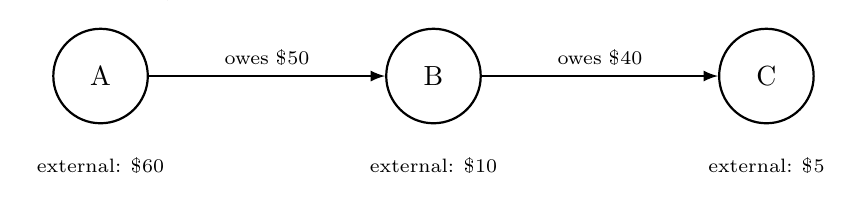
\begin{tikzpicture}[>=latex,thick,node distance=3.0cm]
        \node[draw,circle,minimum size=1.2cm] (a) {A};
        \node[draw,circle,minimum size=1.2cm,right=of a] (b) {B};
        \node[draw,circle,minimum size=1.2cm,right=of b] (c) {C};
        \draw[->] (a) -- node[above,font=\scriptsize] {owes \$50} (b);
        \draw[->] (b) -- node[above,font=\scriptsize] {owes \$40} (c);
        \node[below=0.3cm of a,font=\scriptsize] {external: \$60};
        \node[below=0.3cm of b,font=\scriptsize] {external: \$10};
        \node[below=0.3cm of c,font=\scriptsize] {external: \$5};
    \end{tikzpicture}
\end{bookfigure}

In the baseline, with no shock, every bank pays in full. A's resources are its $\$60$ of external assets (no one owes A anything), covering its $\$50$ obligation to B and leaving A with net worth $60-50=\$10$. B's resources are its $\$10$ of external assets plus the $\$50$ from A, $\$60$ in total, covering its $\$40$ obligation to C and leaving B with net worth $60-40=\$20$. C's resources are its $\$5$ of external assets plus the $\$40$ from B, a net worth of $\$45$. Total system-wide net worth is $10+20+45=\$75$.

Now suppose an external shock, a bad loan or a trading loss unrelated to the interbank network, destroys $\$45$ of Bank A's external assets, leaving A with $\$15$. Recomputing the clearing vector: A's resources are $\$15$ against its $\$50$ obligation, so A pays only $\min(15,50)=\$15$ to B, a default with a $30\%$ recovery rate, leaving A with net worth $\$0$. B's resources are its $\$10$ of external assets plus only $\$15$ from A (not the $\$50$ it was owed), $\$25$ in total, against its $\$40$ obligation to C; B can pay only $\min(25,40)=\$25$, so \emph{B also defaults}\index{default cascade}, with a $62.5\%$ recovery rate, although B suffered no external shock: its default is entirely a consequence of A's. C's resources are its $\$5$ plus only $\$25$ from B (not the $\$40$ it was owed), for a final net worth of $\$30$, down from $\$45$, a real loss even though C owes nothing and never defaults.

Table~\ref{tab:abm-contagion} summarizes the cascade. Total system-wide net worth falls from $\$75$ to $0+0+30=\$30$, a loss of $\$45$, equal to the original shock: the network neither creates nor destroys value, it redistributes one institution's loss across every institution downstream of it, in a pattern invisible to a stress test of Bank A's portfolio alone\index{systemic risk!stress testing}.

\begin{booktable}[htbp]{The default cascade following a \$45 shock to Bank A's external assets (all figures in \$)}{tab:abm-contagion}
\begin{tabular}{lrrrrrr}
\toprule
Bank & External (shocked) & Owed & Received & Paid & Net worth (baseline) & Net worth (shocked) \\
\midrule
A & 15 & 50 & 0  & 15 & 10 & 0 \\
B & 10 & 40 & 15 & 25 & 20 & 0 \\
C & 5  & 0  & 25 & 0  & 45 & 30 \\
\bottomrule
\end{tabular}
\end{booktable}

\vignetteheading{\subsection}{ramsi}{The Bank of England's RAMSI Model}
\index{Bank of England RAMSI model}

The contagion mechanism worked by hand in Section~\ref{sec:abm-contagion-worked} is a simplified version of machinery central banks actually use. The Bank of England's RAMSI (the Risk Assessment Model for Systemic Institutions) is a large-scale, top-down stress-testing model of the UK banking sector\index{stress testing!network}: top-down in that the same model and assumptions apply to every major bank, so results can be compared across banks and added up to a view of the whole system. Work on it began before the 2008 financial crisis, whose Gaussian-copula CDO mispricing Chapter~\chnum{creditrisk} examines; a prototype was presented at central-bank conferences in 2007, and the model was used in the IMF's 2011 assessment of the UK financial sector. Each bank enters with its own balance sheet and income statement, projected forward under macroeconomic scenarios and linked to the others through interbank exposures\index{interbank network}, the network-level cascade of Section~\ref{sec:abm-contagion-worked}'s three-bank example at a far larger scale.

RAMSI is not a full agent-based model in this chapter's sense. Its banks do not optimize, and its developers describe them as acting largely passively: each follows simple behavioral rules, such as a target capital ratio that governs how retained earnings are reinvested. What carries it beyond Section~\ref{sec:abm-contagion-worked}'s clearing vector is a set of feedback effects on top of those rules. A bank whose fundamentals are projected to weaken pays more for funding and, past certain thresholds, is shut out of funding markets altogether\index{liquidity!funding liquidity}, and banks perceived to resemble it face a higher chance of being shut out too. A bank in trouble may also sell assets, pushing down their prices and causing mark-to-market losses at every other bank holding them\index{fire sale}, a channel absent from the pure balance-sheet cascade, where no bank's response could feed back into the market prices other banks' balance sheets depend on. The distinction matters in practice: a pure Eisenberg-Noe network captures what regulators call first-round, direct contagion\index{contagion} (a defaulted counterparty's unpaid obligations), while fire-sale and funding feedbacks capture second-round, indirect contagion (one bank's distress damaging other, still-solvent banks through prices and funding markets), the individually reasonable but collectively destabilizing dynamic of Section~\ref{sec:abm-why}'s Schelling and Flash Crash discussions. In the Bank's prototype these feedbacks turn jointly normal shocks into a bimodal distribution of system-wide outcomes, with a small second peak of contagious defaults in the tail, which neither the three-bank chain nor the hub-and-spoke example, both purely first-round mechanisms, can reproduce.

Models of this kind stress-test the UK banking system as a network rather than one institution at a time, extending Chapter~\chnum{marketrisk}'s single-portfolio framework to the contagious, second-round loss an institution-by-institution stress test misses: in the worked example, a stress test of Bank B alone, which received no direct shock, would have reported B as healthy right up until it wasn't. Other central banks and the IMF have developed comparable network-based systemic-risk tools, some with agent-based behavioral components, and system-wide stress testing is now a standard, if specialized, part of the macroprudential toolkit alongside the single-institution VaR and stress-testing methods of Chapter~\chnum{marketrisk}.

\subsection{Agent-Based Models versus Multi-Agent Reinforcement Learning: Fixed Rules versus Learned Behavior}
\label{sec:abm-vs-marl}\index{multi-agent reinforcement learning!versus agent-based models}

Chapter~\chnum{rl}'s discussion of multi-agent dynamics observes that an agent trained against a static historical simulator implicitly assumes every other participant's behavior stays fixed, an assumption the Flash Crash's hot-potato effect shows can fail badly. Agent-based models and multi-agent reinforcement learning (MARL) are two responses to that observation rather than competitors. An ABM specifies each agent's rule directly (fundamentalist, chartist, zero-intelligence) and asks what emerges from many fixed rules interacting; a MARL system lets each agent's behavior be learned\index{multi-agent reinforcement learning}, typically with Chapter~\chnum{rl}'s Q-learning or policy-gradient machinery, adapting to the others' evolving behavior. The ABM gives up realism about how traders learn in exchange for transparency and tractability, since every rule in this chapter is a single, interpretable equation; MARL gives up that transparency for agents that behave more like real, adaptive participants, at the cost of the training instability and weak convergence guarantees Chapter~\chnum{rl} flags as MARL's central open problem. A growing body of research combines the two, building ABMs in which some or all agents follow reinforcement-learning policies and using the simulated market as the kind of training environment Chapter~\chnum{rl}'s execution and market-making sections rely on, an active research direction rather than a settled methodology. Table~\ref{tab:abm-vs-marl} summarizes the practical trade-offs.

\begin{booktable}[htbp]{Agent-based models (fixed rules) versus multi-agent reinforcement learning (learned behavior)}{tab:abm-vs-marl}
\begin{tabular}{L{3.0cm}L{5.0cm}L{5.6cm}}
\toprule
 & Agent-based model & Multi-agent reinforcement learning \\
\midrule
Agent behavior     & Fixed, hand-specified rule            & Learned via Chapter~\chnum{rl}'s Q-learning or policy-gradient methods \\
Interpretability   & High: every rule is a single, readable equation & Low: behavior is implicit in a trained policy's weights \\
Adaptivity         & None, unless the modeler adds explicit switching (Section~\ref{sec:abm-fundamentalist-chartist}) & Agents adapt continuously to each other's evolving behavior \\
Convergence guarantees & Not applicable; the model is simulated, not trained & Weak once multiple agents learn simultaneously (Chapter~\chnum{rl}) \\
Computational cost & Low to moderate                        & High, and grows sharply with agent count \\
Typical role in this book & Exploring what mechanisms are capable of producing an observed pattern (Section~\ref{sec:abm-calibration}) & Training a single production policy against a realistic simulated environment \\
\bottomrule
\end{tabular}
\end{booktable}

\weheading{\subsection}{abm-learning-seller}{A Learning Seller in the Double Auction}\index{double auction!learning seller}
\label{sec:abm-learning-seller}

To make the ABM-versus-MARL distinction concrete, reconsider Section~\ref{sec:abm-zi}'s double auction, but replace one zero-intelligence seller with a seller who learns, in the trial-and-error spirit of Chapter~\chnum{rl}'s bandit examples\index{multi-armed bandit}. Each round, a new buyer arrives with a valuation drawn from $\{45,50,55,60,65\}$ with equal probability, facing a seller with cost $\$40$ who chooses between two fixed ask levels: Arm H (ask $\$58$) or Arm Lo (ask $\$47$). A trade occurs whenever the ask is at or below the buyer's valuation, earning the seller ask minus cost; a rejected ask earns nothing. The true expected profit of each arm, unknown to the seller but computable from the valuation distribution, is
\begin{align*}
\mathbb{E}[\text{profit}_H] &= \Pr(v\ge 58)\times(58-40) = \tfrac{2}{5}\times18 = 7.2,\\
\mathbb{E}[\text{profit}_{Lo}] &= \Pr(v\ge 47)\times(47-40) = \tfrac{4}{5}\times7 = 5.6,
\end{align*}
so Arm H, despite trading only half as often, is the better arm: its larger profit per trade more than compensates for its lower fill rate, a trade-off that neither arm's trade frequency reveals on its own.

The learning seller explores both arms twice (rounds 1 through 4, alternating H, Lo, H, Lo) and then plays greedily, choosing whichever arm has the higher running-average realized profit. Table~\ref{tab:abm-bandit} traces one representative 12-round history. After the four exploration rounds, Arm H's running average stands at $\$9.00$ against Arm Lo's $\$3.50$, so the seller plays Arm H for the rest of the sequence, the true optimal choice, and its running average, swinging between $\$6.00$ and $\$10.80$ along the way, happens to finish the twelfth round at the true value of $\$7.20$.

\begin{booktable}[htbp]{One 12-round history of the learning seller in the double auction}{tab:abm-bandit}
\begin{tabular}{rrlrrr}
\toprule
Round & Buyer value & Arm played & Profit & Avg.\ profit, H & Avg.\ profit, Lo \\
\midrule
1  & 45 & H  & 0  & 0.00  & --   \\
2  & 45 & Lo & 0  & 0.00  & 0.00 \\
3  & 60 & H  & 18 & 9.00  & 0.00 \\
4  & 55 & Lo & 7  & 9.00  & 3.50 \\
5  & 55 & H  & 0  & 6.00  & 3.50 \\
6  & 60 & H  & 18 & 9.00  & 3.50 \\
7  & 60 & H  & 18 & 10.80 & 3.50 \\
8  & 45 & H  & 0  & 9.00  & 3.50 \\
9  & 55 & H  & 0  & 7.71  & 3.50 \\
10 & 45 & H  & 0  & 6.75  & 3.50 \\
11 & 55 & H  & 0  & 6.00  & 3.50 \\
12 & 65 & H  & 18 & 7.20  & 3.50 \\
\bottomrule
\end{tabular}
\end{booktable}

This is the ABM-versus-MARL distinction of Table~\ref{tab:abm-vs-marl} within a single example: every other seller in Section~\ref{sec:abm-zi} follows a fixed rule (draw a random ask), while this one adapts its behavior to realized experience, the shift from a specified rule to a learned policy that separates the table's two columns. A single 12-round history shows only so much. In this valuation sequence, each arm's first exploration draw met a \$45 buyer and earned nothing, and the deciding second draws went H's way: a \$60 buyer accepted the high ask, while the \$55 buyer facing the low ask earned the seller only \$7. That locked the seller onto the correct arm, but on two observations per arm, a margin far too thin to trust. A less fortunate exploration phase could as easily have left a misleadingly low early estimate for the better arm, favoring the worse one for a while: the explore-exploit tension\index{exploration-exploitation trade-off} that makes reinforcement learning harder in practice than this clean run suggests.

\subsection{Discrete-Choice Switching Replaces the Fixed Threshold}
\label{sec:abm-discrete-choice}\index{Brock-Hommes model!discrete-choice switching}

The learning seller replaces one agent's fixed rule with something learned. The same question applies to Section~\ref{sec:abm-stylized-facts}'s regime-switching market, where the population mix $(n_f,n_c)$ evolved only according to a threshold rule handed down by the modeler (switch to the volatile regime whenever the last price move exceeds a fixed cutoff), not according to anything a fundamentalist or chartist experienced. Brock and Hommes's own mechanism, named in Sections~\ref{sec:abm-why} and~\ref{sec:abm-stylized-facts} and derived in full in this book's companion technical note on the Brock-Hommes model, replaces that external threshold with the comparison a real trader would make: each period, each strategy's population share updates by a discrete-choice (logit) rule driven by that strategy's recently realized profit, so the switching Section~\ref{sec:abm-stylized-facts} imposed from outside emerges from many agents each comparing two numbers and choosing, probabilistically, whichever strategy has recently paid off better.

Reusing Section~\ref{sec:abm-fundamentalist-chartist}'s market, $p_f=100$, $\alpha=0.3$, $\beta=1.0$, $\lambda=1.5$, $p_{-1}=93$, $p_0=95$, define each strategy's realized profit at $t$ as the price change just observed times the demand that strategy would have submitted one period earlier,
\begin{equation*}
\pi_{f,t} = (p_t-p_{t-1})\,d^f_{t-1}, \qquad \pi_{c,t} = (p_t-p_{t-1})\,d^c_{t-1},
\end{equation*}
and update the fundamentalist population share by the binary logit rule
\begin{equation}
n_{f,t} = \frac{e^{\theta \pi_{f,t}}}{e^{\theta\pi_{f,t}}+e^{\theta\pi_{c,t}}}, \qquad n_{c,t}=1-n_{f,t},
\label{eq:abm-logit-switching}
\end{equation}
where $\theta\ge0$ is the intensity of choice (written $\theta$ rather than the technical note's $\beta$, to avoid clashing with this chapter's chartist coefficient $\beta$): $\theta=0$ freezes the population at its starting split regardless of performance, while a large $\theta$ sends nearly the whole population to whichever strategy did even slightly better last period.

Starting from an uninformed $n_{f,0}=n_{c,0}=0.5$, no fitness history yet exists to compare, and $\theta=0.5$, Table~\ref{tab:abm-discrete-choice} works the first three periods by hand.

\begin{booktable}[htbp][Discrete-choice switching in place of a fixed threshold]{Discrete-choice switching ($\theta=0.5$) replacing Section~\ref{sec:abm-stylized-facts}'s fixed threshold. Each period's population shares are computed from the fitness realized over the immediately preceding period, then used to set that period's aggregate demand.}{tab:abm-discrete-choice}
\begin{tabular}{lrrrrrrr}
\toprule
$t$ & $p_t$ & $n_{f,t}$ & $n_{c,t}$ & $d^f_t$ & $d^c_t$ & $D_t$ & $p_{t+1}$ \\
\midrule
0 & 95.000  & 0.500 & 0.500 & 1.500    & 2.000 & 1.750 & 97.625 \\
1 & 97.625  & 0.342 & 0.658 & 0.713    & 2.625 & 1.972 & 100.583 \\
2 & 100.583 & 0.056 & 0.944 & $-0.175$ & 2.958 & 2.783 & 104.757 \\
\bottomrule
\end{tabular}
\end{booktable}

The first period's fitness gap is already informative: with $\Delta p_1=2.625$, the chartist demand submitted the period before, $d^c_0=2.0$, earned a realized profit of $\pi_{c,1}=2.625\times2.0=5.250$, against the fundamentalist's $\pi_{f,1}=2.625\times1.5=3.938$; chartists were not just more numerous but more profitable, since their demand was better aligned with the up-move that materialized. The logit rule converts this into $n_{c,1}=0.658$, already at the edge of the critical threshold\index{fundamentalists and chartists!stability condition} $n_c^{*}\approx0.667$ Section~\ref{sec:abm-stability} derived for the same $\lambda$ and $\beta$. One more period of chartist outperformance, $\pi_{c,2}=7.764$ against $\pi_{f,2}=2.107$, pushes the population past the threshold to $n_{c,2}=0.944$, and the price increments confirm that the market has crossed into the unstable regime: $\Delta p_1=2.625$, $\Delta p_2=2.958$, $\Delta p_3=4.174$, growing rather than shrinking, Scenario B's explosive signature, reached here with no threshold rule in the model, only agents comparing two realized numbers each period and updating a choice probability.

This result fits neither column of Table~\ref{tab:abm-vs-marl} unchanged. It is not Chapter~\chnum{rl}'s Q-learning: no agent maintains a state-action value table or bootstraps a return estimate as the learning seller does. It is a population-level analogue of the same idea, an evolutionary or replicator dynamic in which strategies that recently paid off are used by more of the population next period. That matters for interpretability: a logit population share is a single number a reader can audit by hand, as this worked example did, unlike a trained neural-network policy's weights, so discrete-choice switching sits nearer the transparent, fixed-rule end of the spectrum than the learning seller does, even though both replace a rule the modeler would otherwise impose with something the agents determine. The companion technical note develops the mechanism with a fully specified CARA-utility demand system instead of this chapter's linear demand rules and derives, in closed form, the equilibrium population share and its stability condition as a function of the intensity of choice, an analogue of this section's $n_c^{*}$ expressed as a threshold on $\theta$ rather than on the population share, since in that richer model the share is an endogenous function of $\theta$ rather than a free parameter. Brock and Hommes's result goes further: beyond the critical intensity of choice, the market does not merely become unstable, its dynamics undergo a period-doubling bifurcation into deterministic chaos\index{Brock-Hommes model}, price behavior statistically indistinguishable from noise although generated by a fully deterministic, rational system, the technical note's ``rational route to randomness.'' Readers who want the rigorous derivation should turn to the technical note.

\subsection{When the Agents Are Algorithms: Collusion, Herding, and Supervisory Simulation}
\label{sec:abm-ai-agents}

The learning seller faced buyers who never learned back. Put two learning algorithms in the same market and each becomes part of the other's environment, the multi-agent setting of Table~\ref{tab:abm-vs-marl}, and the outcome can surprise their designers. \textcite{calvano2020artificial} let Q-learning pricing agents, the algorithm of Chapter~\chnum{rl}, compete repeatedly in a standard oligopoly model of price competition. The agents consistently learned to charge prices above the competitive level without communicating with one another\index{algorithmic collusion}, and they sustained those prices the way a cartel would: a price cut by one agent was met by a finite phase of punishment, followed by a gradual return to the high price. The result held under cost and demand asymmetries, different numbers of competitors, and several forms of uncertainty. Nothing in the agents' code mentions cooperation; it emerges from the interaction, which is this chapter's central claim in a form a competition authority must take seriously. Competition law has traditionally looked for evidence of an agreement, and two pricing algorithms that never exchange a message leave none. The finding comes from simulation, and how often it occurs in real markets is still debated, but it is a direct warning for any institution that lets learning algorithms set quotes, loan rates, or deposit rates in a concentrated market.

A second concern runs in the opposite direction: not algorithms that learn to coordinate, but algorithms that are already alike. The Financial Stability Board's November 2024 report on artificial intelligence warned that ``the widespread use of common AI models and data sources could lead to increased correlations in trading, lending, and pricing'' and so amplify market stress \parencite{fsb2024ai}, and the Bank of England's Financial Policy Committee pointed in April 2025 to the risk of ``firms taking increasingly correlated positions and acting in a similar way during a stress, thereby amplifying shocks,'' made worse by reliance on a few vendor-provided models \parencite{boe2025ai}. This is \textbf{herding}\index{herding!AI-driven} produced by a \textbf{model monoculture}\index{model monoculture}, and this chapter has already measured why it matters. The fundamentalist-chartist market stays stable only while the trend-following share stays below $n_c^{*}=1/(\lambda\beta)\approx0.667$; if many firms adopt the same model and that model reacts to a recent price move the same way, the effective $n_c$ is set by the model's adoption rather than by a diversity of independent judgments, and adoption alone can carry it across the threshold. A population's composition is exactly what an agent-based model varies and a representative-agent model cannot, which is why simulating many AI-driven traders is a natural way to study the question.

Central banks have extended the same approach well beyond RAMSI. Bank of England staff built an agent-based model of the UK housing market\index{Bank of England housing-market model} in which first-time buyers, owner-occupiers, buy-to-let investors, and renters are each simulated individually and calibrated to household survey and housing market micro-data \parencite{baptista2016macroprudential}; in it a larger buy-to-let sector amplifies house-price cycles, and a portfolio limit on high loan-to-income mortgages attenuates them, a policy question about population composition that only a heterogeneous-agent model can pose. The Bank's \textbf{system-wide exploratory scenario}\index{system-wide exploratory scenario (SWES)} (SWES), launched in June 2023 and reported on 29 November 2024, went further and used real institutions as the agents \parencite{boe2024swes}. Around 50 firms, banks and non-banks among them, were given a hypothetical scenario, a sudden, sharp, and severe shock to global financial markets triggered by geopolitical tensions, and over several rounds reported how they would respond to it and to one another's responses. The first of the exercise's six conclusions was that firms' collective actions amplify the initial shock. Where Section~\ref{sec:abm-calibration} warns that an agent-based model's behavioral rules are assumptions the modeler must defend, SWES replaced the assumed rules with each participant's own account of its behavior, at the price of an exercise that cannot be rerun at will the way a simulation can.

\section{Building and Validating a Model}

An agent-based model that matches nothing is a simulation, not a model; this part covers the difference.

\subsection{Calibrating and Validating Agent-Based Models}
\label{sec:abm-calibration}\index{agent-based model (ABM)!calibration}\index{calibration!of agent-based models}

Chapter~\chnum{ml} validates a model by holding out data the model never saw and checking its predictions against it, a well-defined procedure because the model makes a specific, checkable prediction for each held-out observation. Agent-based models are far harder to validate in this sense\index{agent-based model (ABM)!validation}: an ABM produces an entire simulated history, and the object of interest is usually a qualitative or statistical property of that history (does it produce fat tails, a plausible contagion cascade?), not a point forecast. The standard approach, the method of simulated moments\index{method of simulated moments}, chooses the model's free parameters (here, $\alpha$, $\beta$, $\lambda$, and the rule governing $n_f$ and $n_c$) so that the simulated data's statistical moments, its volatility, kurtosis, and autocorrelation structure, match the same moments of real market data as closely as possible, rather than maximizing a likelihood as Chapter~\chnum{ml}'s models typically do.

This procedure deserves the skepticism Chapter~\chnum{ml} applies to overfitting\index{overfitting}: an ABM with enough free behavioral parameters can often be tuned to match almost any set of stylized facts, which shows that the model is flexible, not that its mechanism (fundamentalists and chartists switching by relative profitability, say) is the true explanation for those facts. A model that reproduces fat tails is not thereby confirmed; a different ABM, or different parameters in the same one, might reproduce them through an entirely different mechanism. This is a substantive limitation, and the main reason this book uses agent-based models to explore which mechanisms can produce an observed pattern, alongside institutional case studies like the Flash Crash and the RAMSI vignette, rather than as forecasting tools validated the way Chapter~\chnum{ml}'s classifiers and Chapter~\chnum{timeseries}'s time-series models are.

\subsubsection*{Concretely: Matching a Target Moment}\index{method of simulated moments}

Section~\ref{sec:abm-stylized-facts}'s regime-switching simulation happened to produce a Pearson kurtosis of $4.67$ from a switching threshold of $0.25$; nothing forced that value. Method-of-simulated-moments calibration treats the switching threshold (and the model's other free parameters) as a dial to search over, rerunning the simulation at several threshold values and recording the resulting kurtosis, as Table~\ref{tab:abm-msm-sweep} does.

\begin{booktable}[htbp]{Simulated kurtosis as a function of the switching threshold (500 periods, otherwise identical to Section~\ref{sec:abm-stylized-facts})}{tab:abm-msm-sweep}
\begin{tabular}{rr}
\toprule
Switching threshold & Pearson kurtosis \\
\midrule
0.15 & 3.87 \\
0.20 & 3.61 \\
0.25 & 4.67 \\
0.30 & 7.42 \\
0.35 & 8.60 \\
\bottomrule
\end{tabular}
\end{booktable}

The direction is not the one intuition suggests: across the sweep, kurtosis \emph{rises} as the threshold rises, that is, as the volatile regime becomes \emph{harder} to trigger. The rise is not perfectly monotone (kurtosis dips from $3.87$ to $3.61$ between the two lowest thresholds), and the dip is itself instructive: each row is a single $500$-period run, and kurtosis from one short simulated history is noisy enough to reverse a small step, which is why practical method-of-simulated-moments work averages each moment over many seeds before comparing it with data. A low threshold puts the market into the volatile regime often, raising overall variance but blending the two regimes together; a high threshold makes the volatile regime rare, so when it does trigger it produces a few sharp outliers against a calm baseline, the mixture of a common calm regime and a rare extreme one that drives kurtosis up. Suppose an analyst wanted the simulation to match an asset's historical kurtosis of $6.0$: Table~\ref{tab:abm-msm-sweep} brackets the target between the thresholds $0.25$ and $0.30$, which land at $4.67$ and $7.42$, nearly equidistant on either side, so a finer search between them is the next step. Finding a threshold that approximately matches $6.0$ would establish only that this mechanism, among many other threshold values, population-share assumptions, or ABM structures, is \emph{capable} of producing that kurtosis, not that real traders switch strategies by anything like this rule, and, as the reversed direction shows, not that the calibrated parameter's economic interpretation (``how readily the market panics'') behaves as casual intuition suggests. That gap between matching a moment and confirming a mechanism is Section~\ref{sec:abm-calibration}'s central caution, here in computed numbers.

\subsection{Advanced Topics: Network Topology and the Limits of a Simple Chain}
\label{sec:abm-advanced}\index{network topology}

Section~\ref{sec:abm-contagion-worked}'s three-bank example used the simplest possible network, a chain, in which every bank has one creditor and at most one debtor. Real interbank networks look nothing like a chain\index{interbank network}: they are typically core-periphery structures, a few large, heavily interconnected banks at the core surrounded by many smaller banks connected mainly to the core, and the network's shape matters for how a shock propagates, not just its size. Acemoglu, Ozdaglar, and Tahbaz-Salehi's widely cited ``robust-yet-fragile'' result formalizes\index{systemic risk!network models} a counterintuitive finding: for small shocks, a more densely connected network is more stable, since each bank's exposure to any one counterparty's distress is diluted across many relationships, the diversification logic of Chapter~\chnum{portfolio}'s portfolio theory. Past a certain shock size, the same dense interconnection becomes a contagion channel that transmits a large shock further and faster than a sparser network would, because a large loss at one interconnected core bank has many more counterparties to infect.

\weheading{\subsection}{abm-topology}{Chain versus Hub-and-Spoke}\index{network topology!chain versus hub-and-spoke}
\label{sec:abm-topology-worked}

Replace Section~\ref{sec:abm-contagion-worked}'s chain with a hub-and-spoke network hit by the same $\$45$ shock, so the two topologies can be compared. Figure~\ref{fig:abm-topology} sets them side by side. A hub bank $H$ owes $\$30$ to each of three peripheral banks $P_1$, $P_2$, $P_3$ ($\$90$ in total), $H$ holds $\$100$ of external assets, and each $P_i$ holds $\$5$ of external assets and owes nothing. In the baseline, $H$ pays all three in full, leaving $H$ with net worth $100-90=\$10$ and each $P_i$ with $5+30=\$35$, for a total system net worth of $10+3(35)=\$115$.

Now apply the same $\$45$ shock used against Bank A in Section~\ref{sec:abm-contagion-worked}, this time to $H$'s external assets, reducing $H$'s resources to $\$55$ against its $\$90$ obligation. Eisenberg-Noe clearing requires $H$ to pay each equally senior creditor\index{Eisenberg-Noe clearing model} the same pro-rata share: $H$ can cover only $55/90=61.1\%$ of what it owes, so each $P_i$ receives $\$18.33$ instead of $\$30$. $H$'s net worth falls to $55-55=\$0$, a default, as Bank A's did in the chain. But now every peripheral bank absorbs a slice of the loss at once rather than in sequence: each $P_i$ ends with net worth $5+18.33=\$23.33$, down from $\$35$, a $33.3\%$ loss for each of the three. Table~\ref{tab:abm-hub-spoke} summarizes both networks. Total system-wide loss is $\$45$ in both cases, equal to the shock regardless of topology, a general property of this clearing mechanism without bankruptcy costs. Topology does not change how much value a shock destroys; it changes how the loss is distributed. The chain concentrates outright default on two institutions in sequence (A, then B), with C absorbing a modest, once-removed spillover. The hub-and-spoke network concentrates default on a single institution, the hub, while spreading a survivable loss across every peripheral bank at once. No peripheral defaults, since none had an obligation to miss, but all three are meaningfully weaker. Neither topology is simply ``worse.'' Which one a regulator should worry about more depends on whether the greater concern is a few outright failures cascading through a chain of counterparties or one well-connected institution's distress passing a loss to everyone depending on it, the topology-dependent judgment RAMSI-style network models are built to inform.

\begin{bookfigure}[htbp][The same \$45 shock under two topologies]{The same \$45 shock under two topologies. Shaded circles default outright; each arrow gives what is owed and what is actually paid after Eisenberg-Noe clearing. The total loss is \$45 either way, but the chain destroys two institutions one after another while the hub-and-spoke destroys one and weakens three at once.}{fig:abm-topology}
    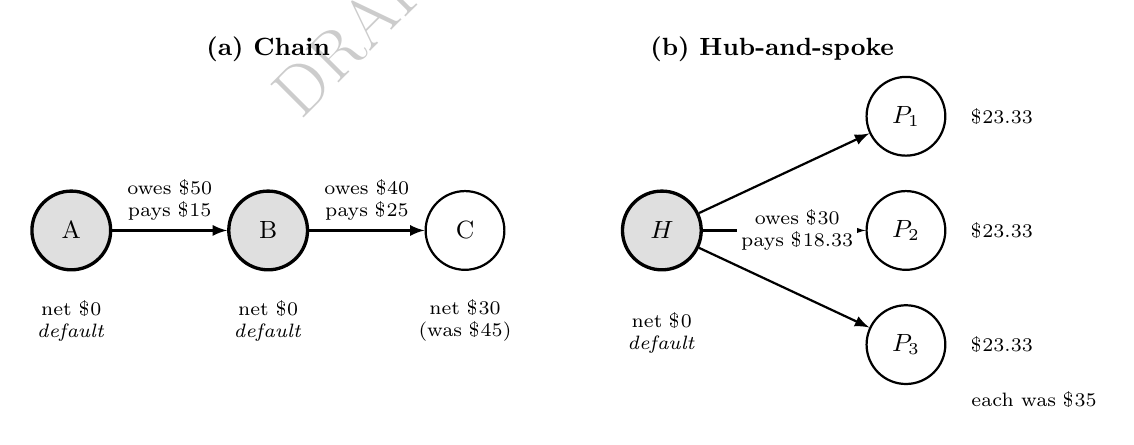
\begin{tikzpicture}[>=latex,thick,
        bank/.style={draw,circle,minimum size=1.0cm,font=\small},
        gone/.style={bank,very thick,fill=gray!25},
        amt/.style={font=\scriptsize,align=center},
        nw/.style={font=\scriptsize,align=center}]
        % (a) the chain of Section 20.2.2
        \node[font=\small\bfseries] at (2.5,2.30) {(a) Chain};
        \node[gone] (a) at (0,0) {A};
        \node[gone] (b) at (2.5,0) {B};
        \node[bank] (c) at (5.0,0) {C};
        \draw[->] (a) -- node[above,amt] {owes \$50\\pays \$15} (b);
        \draw[->] (b) -- node[above,amt] {owes \$40\\pays \$25} (c);
        \node[nw] at (0,-1.15) {net \$0\\\emph{default}};
        \node[nw] at (2.5,-1.15) {net \$0\\\emph{default}};
        \node[nw] at (5.0,-1.15) {net \$30\\(was \$45)};
        % (b) the hub-and-spoke network
        \node[font=\small\bfseries] at (8.9,2.30) {(b) Hub-and-spoke};
        \node[gone] (h) at (7.5,0) {$H$};
        \node[bank] (p1) at (10.6,1.45) {$P_1$};
        \node[bank] (p2) at (10.6,0) {$P_2$};
        \node[bank] (p3) at (10.6,-1.45) {$P_3$};
        \draw[->] (h) -- (p1);
        \draw[->] (h) -- node[pos=0.58,fill=white,inner sep=1.5pt,amt]
            {owes \$30\\pays \$18.33} (p2);
        \draw[->] (h) -- (p3);
        \node[nw] at (7.5,-1.3) {net \$0\\\emph{default}};
        \node[nw,anchor=west] at (11.3,1.45) {\$23.33};
        \node[nw,anchor=west] at (11.3,0) {\$23.33};
        \node[nw,anchor=west] at (11.3,-1.45) {\$23.33};
        \node[nw,anchor=west] at (11.3,-2.15) {each was \$35};
    \end{tikzpicture}
\end{bookfigure}

\begin{booktable}[htbp]{The same \$45 shock, chain versus hub-and-spoke}{tab:abm-hub-spoke}
\begin{tabular}{lrrr}
\toprule
Network & Institutions defaulting outright & Total system loss & Loss distribution \\
\midrule
Chain (Section~\ref{sec:abm-contagion-worked}) & 2 of 3 (A, then B) & \$45 & Concentrated, sequential \\
Hub-and-spoke (above) & 1 of 4 (H only) & \$45 & Diffuse, simultaneous \\
\bottomrule
\end{tabular}
\end{booktable}

A full treatment of the robust-yet-fragile transition would simulate the clearing vector across many more network structures and shock sizes than these two, the large-scale exercise real central-bank network models like RAMSI are built to run.

\subsection{A Practical Workflow for Building an Agent-Based Model}
\label{sec:abm-workflow}\index{agent-based model (ABM)!workflow}

Every example in this chapter, across three different applications (market efficiency, price dynamics, and financial contagion), followed the same workflow. Stated as a template, it is a recipe for building a new ABM and a concrete account of what it means to ask Table~\ref{tab:abm-paradigms}'s question, ``what pattern emerges from many interacting rules,'' rather than fitting a function to data or training a policy against an environment.

\begin{enumerate}
    \item \textbf{Specify the agents and their behavioral rules.} Decide what types of agents populate the model (zero-intelligence traders, fundamentalists and chartists, banks in a network) and write down each type's rule as an explicit function of the current market state, as Sections~\ref{sec:abm-zi} through~\ref{sec:abm-contagion} did with a single equation or a short block of code per agent type.
    \item \textbf{Specify the market mechanism.} Decide how individual agent actions aggregate into a new market state: a double-auction clearing rule, a price-impact equation, an Eisenberg-Noe clearing vector. This is the second box in Figure~\ref{fig:abm-loop}'s simulation loop, and is usually the piece of the model most directly grounded in institutional fact rather than behavioral assumption.
    \item \textbf{Choose free parameters and initial conditions.} Every worked example above had a handful of free parameters, $\alpha$, $\beta$, $\lambda$, the population shares $(n_f,n_c)$, a switching threshold, that are not derived from anything but set by the modeler. Report these explicitly and be prepared to defend each, since Section~\ref{sec:abm-calibration}'s calibration critique applies to every one of them.
    \item \textbf{Simulate forward and collect statistics.} Run the loop for enough periods that the statistic of interest, an efficiency percentage, a variance ratio, a kurtosis, a default count, stabilizes, and report it alongside the raw simulated series wherever possible, as this chapter's companion notebook does for all four worked examples.
    \item \textbf{Calibrate against real data if a real comparison is available.} Where a target real-world moment exists, Section~\ref{sec:abm-calibration}'s method of simulated moments searches over the free parameters from step 3 until simulated and real moments match as closely as possible.
    \item \textbf{Interpret the result as a candidate mechanism, not a confirmed explanation.} A model that reproduces a target pattern has shown that its mechanism is \emph{capable} of producing that pattern; Section~\ref{sec:abm-calibration}'s central caution, the chapter's most important methodological point, is that this is weaker evidence than a validated prediction from Chapter~\chnum{ml}'s train-test framework, and should be presented and used accordingly.
\end{enumerate}

\section{Challenges in Agent-Based Modeling for Finance}

Several challenges explain why ABMs remain a specialized tool rather than a default choice in this book. Computational cost is real: simulating a large, heterogeneous population over many periods, especially when agents are themselves learned with the reinforcement-learning methods of Section~\ref{sec:abm-vs-marl}, can be far more expensive than fitting a closed-form or statistical model. Every worked example here used two to four agents because a hand-checkable illustration must; a research-grade financial ABM typically simulates thousands to millions, and since every agent is updated every period, cost grows at least linearly, and often faster, in both agent count and horizon, a scaling concern this book's other methods (a fitted regression or a trained network) mostly do not share. General-purpose ABM frameworks such as Mesa (Python) and NetLogo exist to manage this complexity, but building and validating a large financial ABM remains a much larger engineering effort than fitting one of Chapter~\chnum{ml}'s models to a comparable dataset. Calibration and validation (Section~\ref{sec:abm-calibration}) remain unresolved: the method of simulated moments can match target statistics without establishing that the mechanism is correct, and there is no counterpart to Chapter~\chnum{ml}'s train-test split for an entire emergent history. Reproducibility across studies is weaker\index{reproducibility} than for most of this book's methods, since two groups' ABMs of nominally the same phenomenon often differ in dozens of rarely specified implementation details (agent count, update order, tie-breaking rules) that can materially change the results. Finally, regulatory and industry acceptance lags the academic literature. RAMSI-style tools have earned a place in the macroprudential toolkit because central banks can defend their assumptions for a narrow, systemic-risk purpose, but agent-based models remain far from routine in the validation and governance framework built around Chapter~\chnum{fraud}'s three lines of defense and Chapter~\chnum{xai}'s explainability toolkit. A rule-based simulation of thousands of interacting agents is harder to explain to a validator or regulator than a fitted regression or classifier.

None of these challenges is a reason to avoid agent-based models; they are reasons to be precise about what a given ABM has shown, the discipline Section~\ref{sec:abm-workflow}'s final step asks for. A model that reproduces the Flash Crash's hot-potato dynamics, the fat tails of Section~\ref{sec:abm-stylized-facts}'s simulation, or RAMSI's contagion cascades is a useful demonstration that a specific, named mechanism is \emph{sufficient} to produce an observed pattern, valuable evidence in its own right and often the only tractable way to reason about emergent phenomena. It is not, on its own, evidence that the mechanism is \emph{necessary}, the one true explanation among the many candidates that might produce the same pattern, and every application in this chapter should be read with that distinction in mind.

\notocsection{Key Takeaways}

\begin{itemize}
    \item Agent-based models simulate a population of heterogeneous, boundedly rational agents interacting repeatedly, and treat the aggregate pattern that emerges, efficiency, a bubble, a cascade, as the object of study, in contrast to this book's representative-agent equilibrium models and data-fitted statistical models.
    \item Market efficiency can emerge from a trading mechanism itself rather than from participant sophistication: zero-intelligence traders bidding at random within budget constraints, cleared through an ordinary double auction, recovered the fully efficient trade in this chapter's worked example.
    \item The same market mechanism can produce either smooth convergence to fundamental value or a self-reinforcing, explosive bubble, depending only on the population mix of fundamentalist and chartist traders, holding every other parameter fixed.
    \item Heterogeneous-agent models can reproduce fat tails and volatility clustering as an emergent consequence of strategy switching, rather than by directly imposing an autoregressive variance structure the way Chapter~\chnum{timeseries}'s GARCH models do: this chapter's 500-period simulation produced a $6.14\times$ variance ratio between regimes, a Pearson kurtosis of $4.67$ against a Gaussian benchmark of $3.0$, and a squared-return autocorrelation of $0.658$ at lag one, from two fixed behavioral rules switching in and out of dominance.
    \item A clearing-vector approach to interbank obligations, the same network-contagion logic at the core of the Bank of England's top-down RAMSI stress-testing model, can show one institution's shock cascading into a second institution's default even when the second institution received no direct shock, a systemic risk a single-institution stress test cannot see.
    \item Agent-based models are far harder to calibrate and validate than this book's other methods, since matching a target set of statistical moments demonstrates flexibility, not that the model's particular mechanism is the true explanation for the observed pattern.
    \item Network topology shapes contagion independently of shock size: the ``robust-yet-fragile'' result shows dense interconnection dampens small shocks through diversification but can transmit large shocks further and faster than a sparser network would; the same \$45 shock produced two outright defaults in a chain network but only one, spread more diffusely, in a hub-and-spoke network of the same total size.
    \item The fundamentalist-chartist market's stability is governed by a single exact threshold, $n_c^{*}=1/(\lambda\beta)$: below it the price converges, above it a bubble grows without bound, and near it convergence becomes oscillatory rather than smooth, a sharp regime change from one parameter crossing a critical value.
    \item Agent-based models answer a third kind of question this book's other two paradigms do not: not ``what function best fits this data'' (Chapter~\chnum{ml}) or ``what action sequence maximizes reward in this environment'' (Chapter~\chnum{rl}), but ``what pattern emerges when many simple, interacting rules are simulated together.''
    \item Even a calibrated parameter's economic interpretation can run against intuition: raising the fundamentalist-chartist model's switching threshold, making the volatile regime \emph{harder} to trigger rather than easier, raised simulated kurtosis from $3.87$ to $8.60$ across a parameter sweep, the opposite of what naive intuition suggests, which is why a calibrated ABM's mechanism should never be trusted just because its output moments look right.
    \item A fixed-rule ABM and a learning agent can share the same market: replacing one zero-intelligence seller with a simple trial-and-error learner that tracks realized profit converged on the true better strategy in this chapter's worked example, but a single unlucky exploration phase can just as easily lock a purely greedy learner onto the wrong one permanently, with no further exploration to self-correct it.
    \item A market's switching threshold can be crossed by assumption or by learning: Section~\ref{sec:abm-stylized-facts}'s regime switch was a rule the modeler imposed from outside, while Section~\ref{sec:abm-discrete-choice}'s discrete-choice mechanism let the population cross the same $n_c^{*}\approx0.667$ threshold on its own, because agents kept reallocating toward whichever strategy had just earned more, reaching $n_{c,2}=0.944$ and an accelerating price after only two periods of chartist outperformance.
    \item When the agents are themselves learning algorithms, emergence cuts both ways: Q-learning pricing agents can learn to collude without communicating, and many firms relying on the same AI models can herd, the population-composition risk that the FSB and the Bank of England now flag and that agent-based models, including the Bank's housing-market model and its system-wide exploratory scenario, are built to study.
\end{itemize}

\notocsection{Suggested Exercises}

\begin{enumerate}[exercises]
    \item Using the zero-intelligence double-auction setup of Section~\ref{sec:abm-zi}, suppose buyer 2's random bid is $b_2=\$49$ instead of $\$30$, with every other draw unchanged. Recompute the clearing outcome and explain, in terms of total realized surplus, whether the market mechanism still selects the efficient allocation.
    \item Section~\ref{sec:abm-stability} derives the stability threshold $n_c^{*}=1/(\lambda\beta)$ for $\lambda=1.5$, $\beta=1.0$. Recompute $n_c^{*}$ for $\beta=2.0$ instead, holding $\lambda=1.5$ fixed, and use the companion notebook to confirm your answer by simulating the market just above and just below the new threshold.
    \item Extend the three-bank contagion network of Section~\ref{sec:abm-contagion-worked} by adding a fourth bank, D, to whom Bank C owes \$20, with D holding \$15 of external assets and no other obligations. Recompute the clearing vector under the same \$45 shock to Bank A's external assets, and report whether the cascade reaches D.
    \item Section~\ref{sec:abm-topology-worked}'s hub-and-spoke example used three peripheral banks. Redo the calculation with six peripheral banks instead, keeping the hub's total obligation at \$90 (so each peripheral is now owed \$15) and its external assets at \$100, under the same \$45 shock. Report each peripheral's percentage loss and compare it to the three-peripheral case's $33.3\%$, and explain the direction of the difference.
    \item Section~\ref{sec:abm-calibration} argues that matching a target set of statistical moments does not confirm an ABM's underlying mechanism. Propose one additional form of evidence, beyond matching moments, that would make you more confident a particular agent-based mechanism is the right explanation for an observed market phenomenon.
    \item Using the companion notebook's regime-switching simulation, lower the switching threshold from $0.25$ to $0.15$ and re-run the $500$-period simulation. Report the new variance ratio and kurtosis, and explain, in terms of how often the market now enters the volatile regime, why the direction of the change makes sense.
    \item Section~\ref{sec:abm-learning-seller}'s learning seller happened to settle on the better arm after exploring. Recompute its running averages after exploration if rounds 1 through 4 instead see buyer values $50, 50, 50, 50$ (using the companion notebook to check your work), report which arm the seller would then play for the rest of the sequence, and explain why this outcome is a failure of the explore-exploit process rather than merely bad luck that later self-corrects.
    \item Using Section~\ref{sec:abm-discrete-choice}'s discrete-choice market, recompute $n_{f,1}$, $n_{c,1}$, $n_{f,2}$, and $n_{c,2}$ with a lower intensity of choice, $\theta=0.2$ instead of $0.5$, holding every other parameter and the same $p_{-1}=93$, $p_0=95$ fixed, and report the first period at which $n_{c,t}$ exceeds the critical threshold $n_c^{*}\approx0.667$ derived in Section~\ref{sec:abm-stability}, comparing it to the $\theta=0.5$ case worked in the text. Does halving the intensity of choice postpone the crossing, change its severity, or both?
    \item Section~\ref{sec:abm-ai-agents} links model monoculture to the stability threshold of Section~\ref{sec:abm-stability}. Suppose a fraction $m$ of a market's participants adopt the same AI trading model, which behaves exactly like a chartist with $\beta=1.0$, while the remaining participants keep Scenario A's split of $80\%$ fundamentalists and $20\%$ chartists, with $\lambda=1.5$. (a) Write the market's chartist share $n_c$ as a function of $m$ and find the smallest adoption rate $m$ at which the market becomes unstable. (b) Repeat with the remaining participants split $90\%$ and $10\%$, and explain what the comparison says about whether diversity among the non-adopters protects the market. (c) Explain why the Bank of England's system-wide exploratory scenario asked participating firms to report their own responses rather than assigning them behavioral rules, and name one limitation of that design relative to a simulation.
    \item \textbf{Challenge (real data).} Download the BIS locational banking statistics (the cross-border claims table, freely available at stats.bis.org with no registration required) for five or six reporting countries. (a) Treating each country's aggregate cross-border claims on the others as a simplified interbank exposure network, construct a liabilities matrix analogous to Section~\ref{sec:abm-contagion-worked}'s three-bank example (using each country's claims on another as that other country's liability), and compute the Eisenberg-Noe clearing vector following an assumed shock that wipes out 10\% of one country's external, non-interbank assets. (b) Compare the resulting loss cascade to this chapter's toy three-bank result, and discuss whether the real network's exposures look more chain-like or more hub-and-spoke, referencing Section~\ref{sec:abm-topology-worked}'s topology comparison. (c) Explain one specific way in which country-aggregated BIS data understates the fragility of the true institution-level network (for example, netting across many banks within a country, or omitting domestic interbank exposures entirely), and describe, referencing this chapter's RAMSI case vignette, what institution-level supervisory exposure data a central bank could use to close that gap.
\end{enumerate}

\notocsection{Further Reading}

\begin{itemize}
    \item \frcite{schelling1971dynamic} The original checkerboard segregation model discussed in Section~\ref{sec:abm-why}, the earliest and best-known agent-based model outside finance.
    \item \frcite{arthur1997asset} The Santa Fe Institute Artificial Stock Market discussed in Section~\ref{sec:abm-why}, widely regarded as the founding model of agent-based computational finance.
    \item \frcite{gode1993allocative} The original zero-intelligence double-auction result worked through by hand in Section~\ref{sec:abm-zi}.
    \item \frcite{brock1997rational} The performance-based strategy-switching framework underlying Section~\ref{sec:abm-fundamentalist-chartist}'s fundamentalist-chartist model.
    \item \frcite{lux1999scaling} An influential heterogeneous-agent model reproducing fat tails and volatility clustering, discussed in Section~\ref{sec:abm-stylized-facts}.
    \item \frcite{eisenberg2001systemic} The clearing-vector framework for financial contagion worked through by hand in Section~\ref{sec:abm-contagion-worked}.
    \item \frcite{acemoglu2015systemic} The ``robust-yet-fragile'' network-topology result discussed in Section~\ref{sec:abm-advanced}.
    \item \frcite{zhang2021multi} A survey of the multi-agent reinforcement learning methods contrasted with fixed-rule agent-based models in Section~\ref{sec:abm-vs-marl}, including the convergence difficulties that arise once multiple agents learn simultaneously.
    \item \frcite{burrows2012ramsi} The real-world central-bank stress-testing model, top-down and network-based, discussed in the case vignette above.
    \item \frcite{calvano2020artificial} The simulation study, discussed in Section~\ref{sec:abm-ai-agents}, in which Q-learning pricing agents learn to sustain supracompetitive prices without communicating.
    \item \frcite{boe2024swes} The Bank of England's report on its system-wide exploratory scenario, in which around 50 real firms played the agents of a market-stress simulation.
    \item \frcite{axtell2025agent} A comprehensive, up-to-date survey of the field from two of its leading figures, and the best single starting point for a reader who wants to go beyond this chapter's introductory treatment.
    \item \frcite{lebaron2006agent} An earlier survey of the agent-based finance literature specifically, including the calibration and validation challenges raised in Section~\ref{sec:abm-calibration}.
    \item \frcite{farmer2009economy} An argument, from two leading practitioners, for agent-based approaches as a complement to equilibrium modeling in macroeconomics and finance.
\end{itemize}

\end{document}

